\section{Sewer construction}\label{se:sewer_construction}
Typically the water treatment plant are constructed near rivers or fjord which is typical at a lower geographical location, thereby enabling the force of the gravity to transport the wastewater in a sewer. If the industry or the households are at a lower geographical location than the water treatment plant, then pumps are used to transport the wastewater as illustrated in figure \ref{fig:Sewer_drawing}.
\begin{figure}[H]
\centering
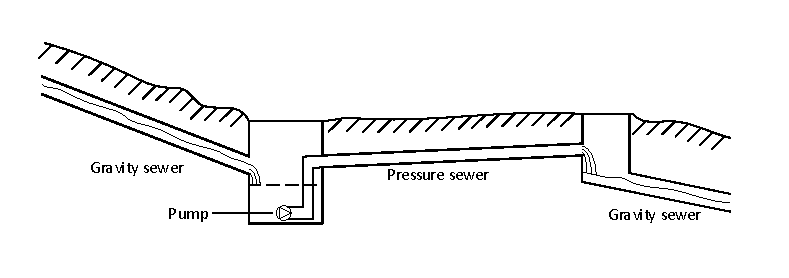
\includegraphics[width=1\textwidth]{report/introduction/pictures/Sewer_drawing.pdf}
\caption{Illustrate different methods for transportation of wastewater.}
\label{fig:Sewer_drawing}
\end{figure}

The pipes are most often constructed in concrete or polyethylene. Where concrete pipes are used for gravity sewers and polyethylene are used in a pressure sewer due to a lower roughness height which means that the friction is less in a polyethylene pipe. 